\chapter{緒論}
\renewcommand{\baselinestretch}{10.0} %設定行距
\pagenumbering{arabic} %設定頁號阿拉伯數字
\setcounter{page}{1}  %設定頁數
\fontsize{14pt}{2.5pt}\sectionef

\section{研究動機與背景}
材料分析軟體的應用在機械領域愈來越廣泛,能夠將繪製零件進行分析,但卻鮮少人知道材料分析是怎麼進行的,背後所引用的代碼、原理的東西。本專題研究方向將由四足機器人作為設計主題,提供所需參數,將有限元素分析的公式套入並計算,對建模進行力學分析,用於設計優化,將透過本專題了解。(圖.\ref{fig.pong_gym})。\\
------------------------------------------------------
\begin{figure}[hbt!]
\begin{center}
\includegraphics[angle=90,width=10cm]{冰球機}
\caption{\Large 實體的冰球機}\label{fig.冰球機}
\end{center}
\end{figure}
-------------------------------------------------------
\begin{figure}[hbt!]
\begin{center}
\includegraphics[angle=90,width=10cm]{origin}
\caption{\Large 虛擬環境簡化後的冰球機}\label{fig.模擬冰球機}
\end{center}
\end{figure}
---------------------------------------------------------
\begin{figure}[hbt!]
\begin{center}
\includegraphics[height=8cm]{pong_gym}
\caption{\Large Gym的Pong game}\label{fig.pong_gym}
\end{center}
\end{figure}
--------------------------------------------------------------

\section{研究目的與方法}
本專題研究是以有限元素法有限元分析,Solid Edge繪出3D模型,並加入材質及各式力,測試不同部位所得出的物體模型的模擬分析,求出各個物理問題(應力、應變、變形等)。\\

以四足機械狗為模型,由solid edge建立3D模型,導入CoppeliaSim模擬環境,透過軟體的模擬功能,測試模型可行性,找出機器狗在運動時各部位的軌跡並找出反力為何。\\

接著利用Solid Edge分析,利用軟體中的有限元素法及各式方程式結合成的線性方程、進行代數求解、模擬,觀察、分析此模型在受力後的反應,篩選出適合的材料及形狀,透過此部分驗證材料的性質是否能夠負荷並擁有某些脆弱點,透過以上步驟可驗證實際運用上的此設計是否可行也可以讓設計者盡早發現錯誤並修正。\\
 -------------------------------------------------------------
\begin{figure}[hbt!]
\begin{center}
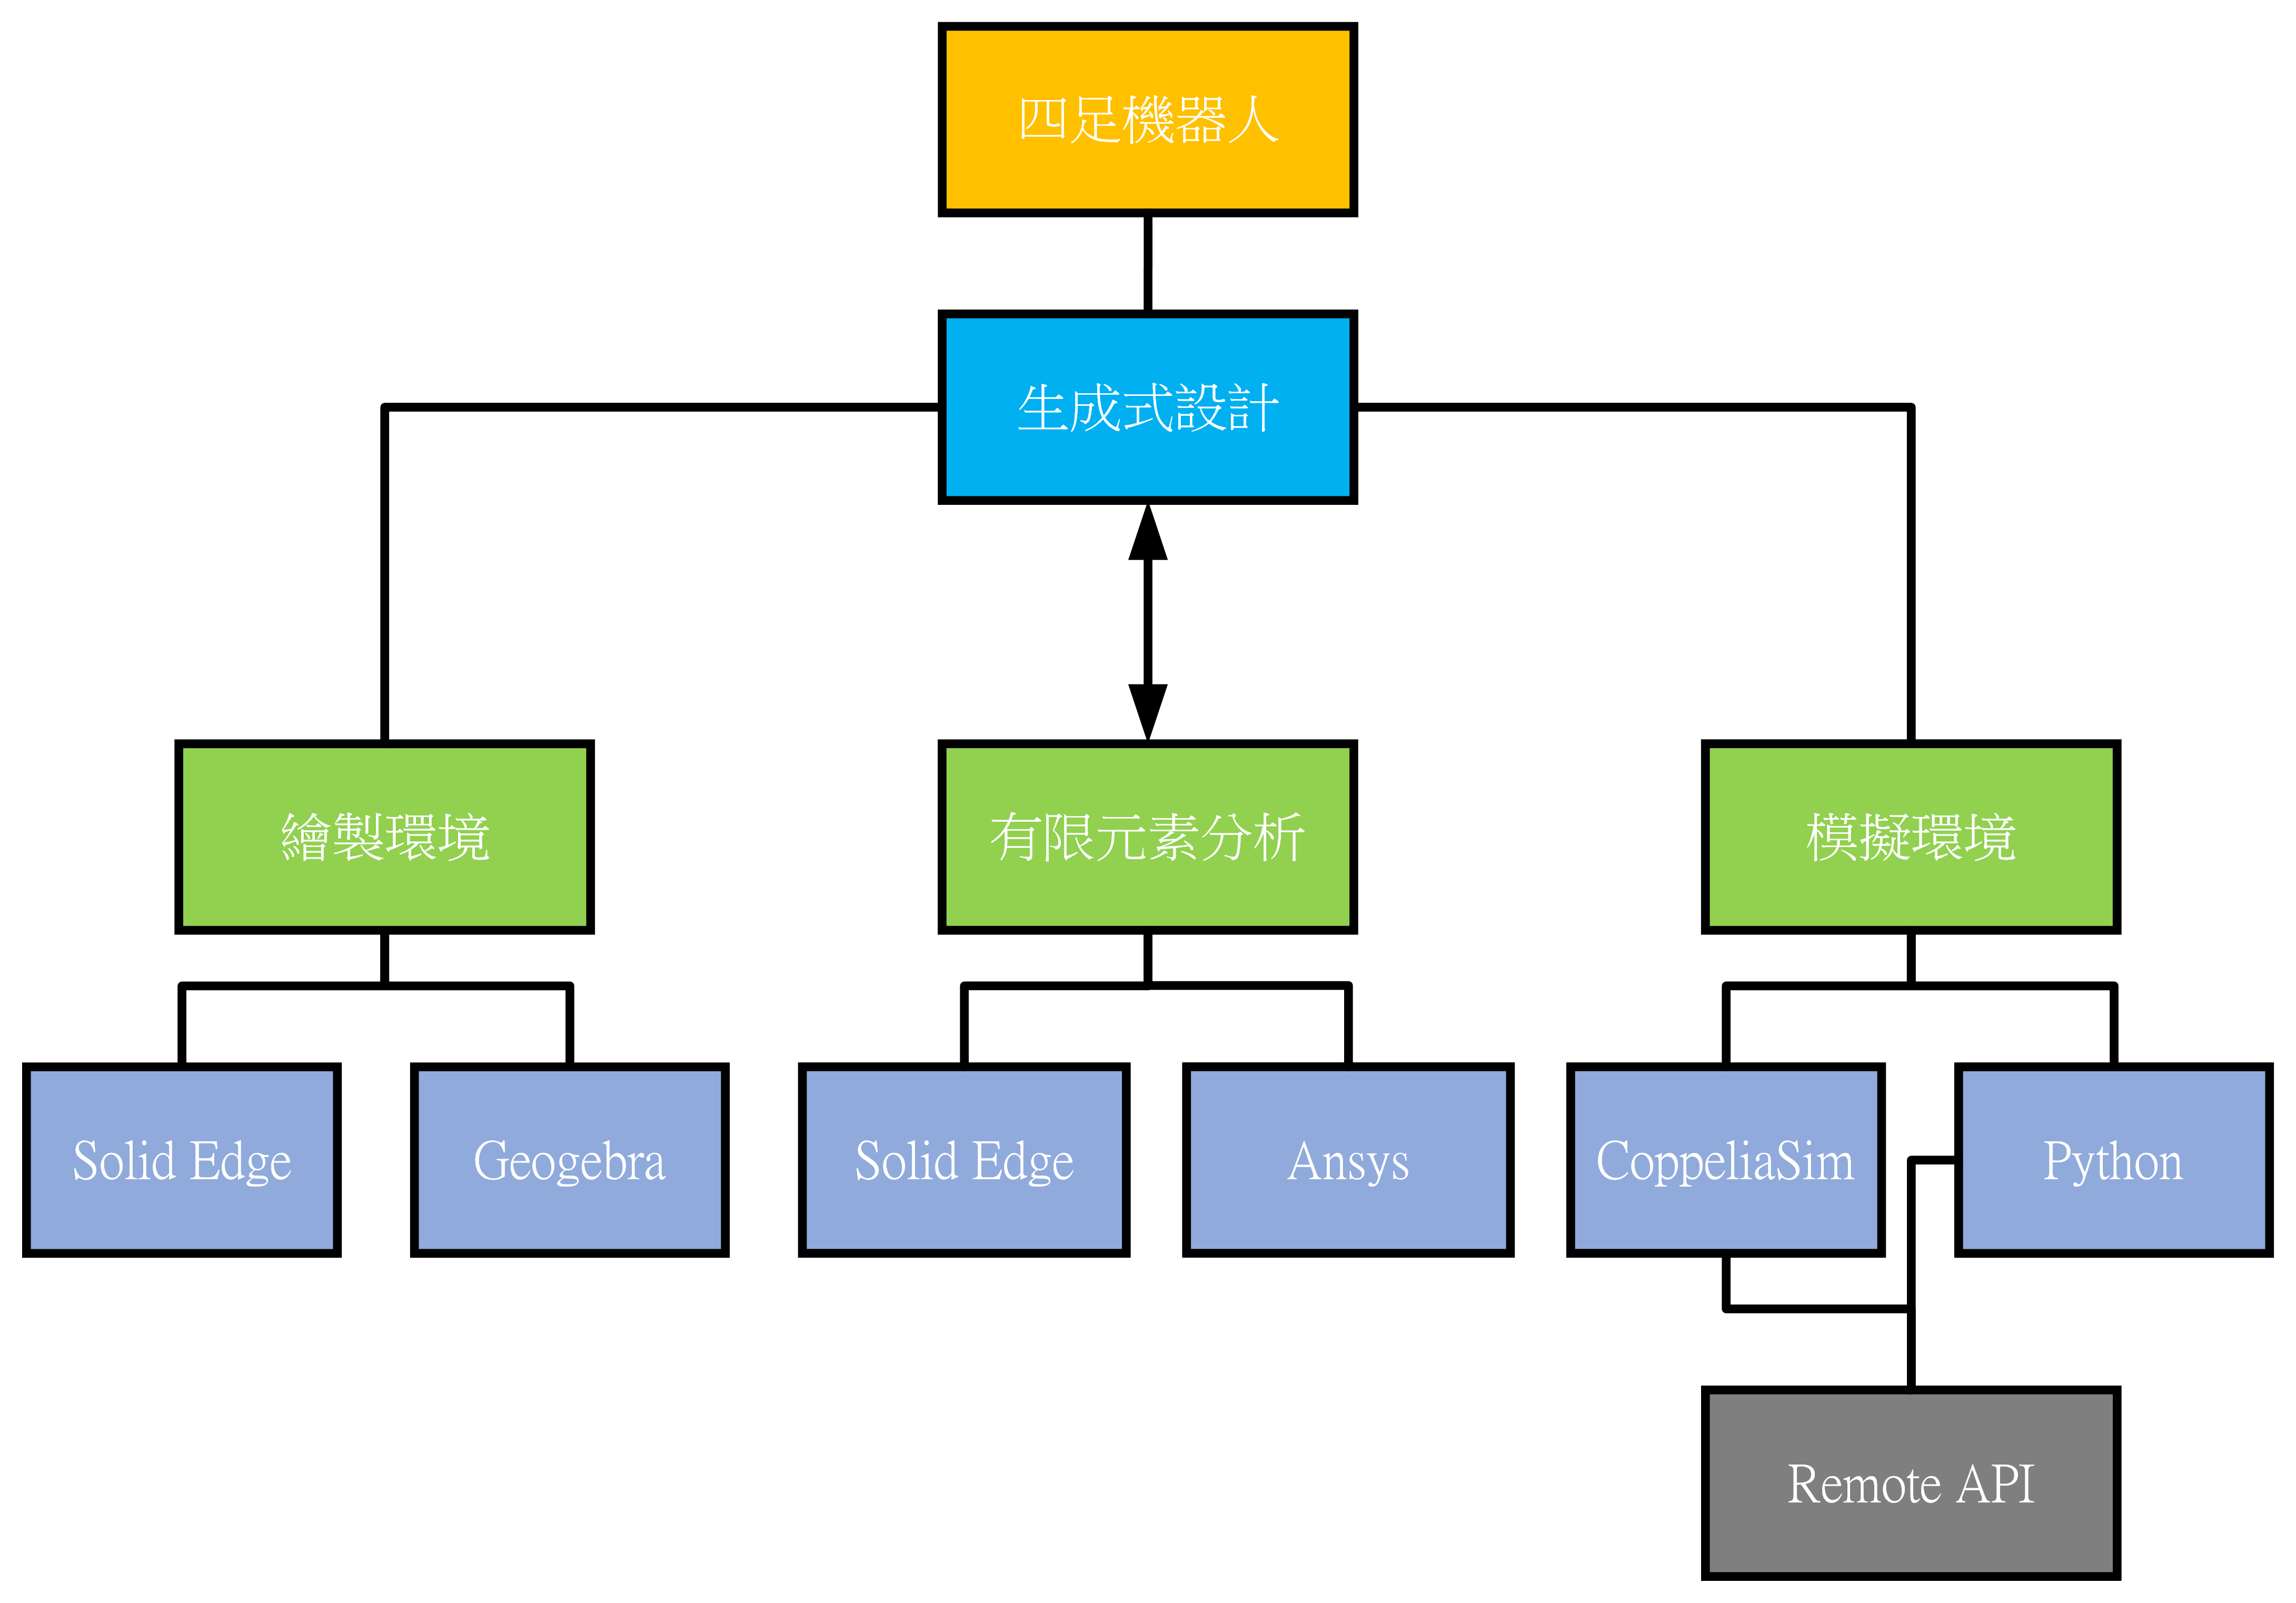
\includegraphics[width=15cm]{研究架構}
\caption{\Large 研究架構 }
\label{研究架構 }
\end{center}
\end{figure}
-------------------------------------------------------

\section{未來展望}

透過此研究可以求解出模型所受外力影響的數值變化,若之後可以對軟體輸入參數及設計因子,則軟體可以在所設定的範圍中透過計算產生設計者所需的模型並且,不再只局限於設計者的想像力,或是透過手機的日漸進步的激光雷達掃描系統,可以讓許多用戶都可以輕易地使用分析功能。\\

\section{分析說明}

模型進行運動分析後,透過求出的反力做為設計參數,帶入到至應力分析軟體中,並帶入合適的材料,通過預設的安全係數為最終目標。\\

\renewcommand{\baselinestretch}{0.5} %設定行距
